\documentclass[12pt,a4paper,fontset=none]{ctexart}

\usepackage[a4paper,left=2.7cm,right=2.7cm,top=2.9cm,bottom=2.8cm,headheight=18pt,footskip=26pt]{geometry}
\usepackage{fontspec}
\usepackage{xeCJK}
\usepackage{microtype}
\usepackage{setspace}
\usepackage{indentfirst}
\usepackage{graphicx}
\usepackage{booktabs}
\usepackage{array}
\usepackage{tabularx}
\usepackage{longtable}
\usepackage{float}
\usepackage{caption}
\usepackage{enumitem}
\usepackage{hyperref}
\usepackage{xurl}
\usepackage{fancyhdr}
\usepackage{lastpage}
\usepackage{titlesec}
\usepackage[most]{tcolorbox}
\usepackage{fvextra}
\usepackage{ragged2e}
\usepackage{etoolbox}
\usepackage{calc}

\IfFontExistsTF{Times New Roman}{\setmainfont{Times New Roman}}{\setmainfont{TeX Gyre Termes}}
\IfFontExistsTF{Songti SC}{\setCJKmainfont{Songti SC}}{\setCJKmainfont{FandolSong}}
\IfFontExistsTF{PingFang SC}{\setCJKsansfont{PingFang SC}}{\setCJKsansfont{FandolHei}}
\IfFontExistsTF{Menlo}{\setmonofont{Menlo}}{\setmonofont{Courier New}}
\IfFontExistsTF{PingFang SC}{\setCJKmonofont{PingFang SC}}{\setCJKmonofont{FandolFang}}

\definecolor{RUCRed}{HTML}{971F30}
\definecolor{RUCSoft}{HTML}{F7F1F2}
\definecolor{Ink}{HTML}{2B2325}
\definecolor{Muted}{HTML}{6D6063}
\definecolor{Line}{HTML}{D9CCD0}
\definecolor{CodeBG}{HTML}{FBF8F7}
\definecolor{LinkBlue}{HTML}{1F5A7A}

\setstretch{1.32}
\setlength{\parindent}{2em}
\setlength{\parskip}{0.35em}
\setlength{\emergencystretch}{3em}
\widowpenalty=10000
\clubpenalty=10000
\displaywidowpenalty=10000

\setcounter{secnumdepth}{0}
\setcounter{tocdepth}{2}
\renewcommand{\contentsname}{目录}
\setlist[itemize]{leftmargin=2.2em,itemsep=0.2em,topsep=0.4em}
\setlist[enumerate]{leftmargin=2.2em,itemsep=0.2em,topsep=0.4em}

\hypersetup{
  colorlinks=true,
  linkcolor=RUCRed,
  urlcolor=LinkBlue,
  citecolor=RUCRed,
  pdftitle={中国环境政策文本结构化抽取预调研报告},
  pdfauthor={环境政策项目},
  pdfsubject={预调研报告},
  pdfcreator={LaTeX build pipeline}
}
\urlstyle{same}

\pagestyle{fancy}
\fancyhf{}
\fancyhead[L]{\small\color{Muted}中国环境政策文本结构化抽取预调研报告}
\fancyhead[R]{\small\color{Muted}2026年4月21日}
\fancyfoot[C]{\small\color{Muted}\thepage}
\renewcommand{\headrulewidth}{0.4pt}
\renewcommand{\footrulewidth}{0pt}

\titleformat{\section}
  {\zihao{-3}\bfseries\color{RUCRed}}
  {}
  {0pt}
  {}
\titleformat{\subsection}
  {\zihao{4}\bfseries\color{Ink}}
  {}
  {0pt}
  {}
\titlespacing*{\section}{0pt}{2.2ex plus .3ex minus .2ex}{1.1ex}
\titlespacing*{\subsection}{0pt}{1.6ex plus .2ex minus .2ex}{0.6ex}

\captionsetup{
  font={small},
  labelfont={bf,color=RUCRed},
  textfont={small},
  skip=8pt
}

\newcolumntype{L}[1]{>{\RaggedRight\arraybackslash}p{#1}}
\newcolumntype{C}[1]{>{\Centering\arraybackslash}p{#1}}
\providecommand{\tightlist}{\setlength{\itemsep}{0pt}\setlength{\parskip}{0pt}}

\DefineVerbatimEnvironment{CodeBlock}{Verbatim}{
  fontsize=\small,
  breaklines=true,
  breaksymbolleft={},
  frame=single,
  rulecolor=\color{Line},
  framesep=4mm,
  baselinestretch=1.0,
  formatcom=\color{Ink}
}

\newtcolorbox{MetaBox}{
  enhanced,
  colback=RUCSoft,
  colframe=RUCRed,
  boxrule=0.8pt,
  arc=2pt,
  left=8pt,
  right=8pt,
  top=8pt,
  bottom=8pt
}

\begin{document}

\begin{titlepage}
\thispagestyle{empty}
\centering
\vspace*{2.8cm}

{\zihao{2}\bfseries\color{RUCRed}中国环境政策文本结构化抽取预调研报告\par}
\vspace{0.9cm}
{\zihao{-3}\color{Ink}基于 50 份环境政策文本与多模型交叉抽取结果的阶段性分析\par}

\vspace{1.8cm}

\begin{minipage}{0.88\textwidth}
\begin{MetaBox}
\renewcommand{\arraystretch}{1.25}
\begin{tabularx}{\textwidth}{>{\bfseries}l X}
版本时间 & 2026年4月21日 \\
结果版本 & \path{llm_results/all_results_summary.json}（2026-04-21 06:29） \\
 & \path{llm_results/all_raw_results.json}（2026-04-21 06:33） \\
图表版本 & \path{output/figures/prestudy_report/}（2026-04-21 07:22） \\
工作属性 & 可追溯版本，用于阶段汇报、专家讨论与正式研究推进 \\
\end{tabularx}
\end{MetaBox}
\end{minipage}

\vfill
{\large\color{Ink}环境政策项目工作底稿\par}
\vspace{0.3cm}
\vspace{1.2cm}
{\normalsize\color{Muted}2026年4月21日\par}
\end{titlepage}

\pagenumbering{Roman}
\tableofcontents
\clearpage
\pagenumbering{arabic}

\section*{摘要}
\addcontentsline{toc}{section}{摘要}

本轮预调研以 50 份中国环境政策文本为对象，覆盖 2009---2024 年，调用
DeepSeek-V3.2、Kimi-K2.5 与 MiniMax-M2.5
三个模型进行平行抽取与交叉比对，并在结果层保留模型一致率、文本来源、失败状态与原始输出轨迹。总体来看，当前抽取流程已经能够稳定识别政策层级、政策力度、政策语气、政策类型、规制严格度、目标层次与政策工具等结构化属性；对执行机制、关键措施、量化目标、创新点、纵向协调等开放式字段，则更适合作为后续规则化构造与人工核验的对象，而不宜直接进入正式计量分析。

从预调研样本本身看，命令控制型与信息公开型工具构成中国环境政策文本的基础骨架，经济激励型工具已广泛嵌入，市场机制型工具则明显依赖具体政策场景；结果型文件的约束性目标更密集、规制强度更高，过程型文件则承载了更多执行安排；《中华人民共和国环境保护法》在样本中构成最重要的上位法锚点。综合判断，本轮预调研已经完成了三个关键任务：一是证明这套多模型抽取方案可以形成可复核的结构化结果；二是明确哪些变量已经可以扩样，哪些变量必须先做二次构造；三是为正式研究中的``中央信号如何进入政策文本、地方如何在文本中完成适配或复制''提供了可靠的测量起点。

\section{一、预调研目标与样本范围}

本轮预调研围绕三个问题展开：第一，现有政策文本能否被稳定、可审计地结构化；第二，哪些变量已经具备进入正式样本扩展的条件；第三，预调研样本自身是否已经呈现出足以支持正式研究设计的经验结构。

纳入样本的 50
份文件覆盖法律、行政法规、部门规章、规范性文件与地方性法规等多类政策文本，时间范围为
2009---2024 年。其中，中央层级文件 43 份，省级文件 6 份，市级文件 1
份；原生可提取文本 47 份，基于官方网页补源的
\path{official\_html\_rescue} 文件 3
份。样本并不追求统计意义上的全国完备覆盖，而是服务于方法检验、变量筛选和正式扩样前的质量判断。

表 1 汇总了本轮预调研的基础事实。

\begin{table}[H]
\centering
\caption{预调研样本基础事实}
\label{tab:basic_facts}
\begin{tabular}{L{0.58\linewidth}C{0.20\linewidth}}
\toprule
指标 & 数值 \\
\midrule
样本文件数 & 50 \\
时间范围 & 2009---2024 \\
中央 / 省级 / 市级 & 43 / 6 / 1 \\
原生文本 / 官方补源 & 47 / 3 \\
平均总体一致率 & 0.593 \\
成功 / 部分成功 & 49 / 1 \\
平均规制严格度 & 4.48 \\
\bottomrule
\end{tabular}
\end{table}

\section{二、数据处理流程与可追溯性安排}

本轮结果采用``文本来源审计---多模型并行抽取---结果汇总---一致率评估---人工核验入口''五步流程。原始政策
PDF 保持不覆盖；对于 3 份原 PDF
不可直接搜索的文件，项目保留官方网页快照与对应纯文本，以
\path{text\_source=official\_html\_rescue}
进入同一套抽取流程。模型输出不仅保留最终汇总值，也保留各模型的原始结果、一致率与失败状态，从而使后续复核不必回到黑箱状态。

在模型层面，三模型平均有效返回数为 2.98，平均失败模型数仅为 0.02；50
份文件中有 49 份达到 \path{success}，仅 1 份为
\path{partial\_with\_failures}。从模型置信度看，Kimi-K2.5 平均置信度为
0.764，DeepSeek-V3.2 为 0.740，MiniMax-M2.5 为
0.729。更重要的是，这轮结果已经能够把``字段本身不稳''和``模型偶发失败''区分开来：前者主要集中在开放式长文本字段，后者则仅见于个别文件。

为支撑后续人工核验，项目已同步刷新
\path{data/metadata/pilot\_validation\_sheet.csv}，形成 10
份重点文件、5 个关键字段、共 50
条记录的核验长表。该表目前已可直接进入人工复核，不再需要重新整理字段或回溯来源。

\section{三、样本结构：政策文本自身呈现出的经验事实}

从样本构成看，政策文本已经表现出相当稳定的制度风格分布。

\begin{figure}[H]
\centering
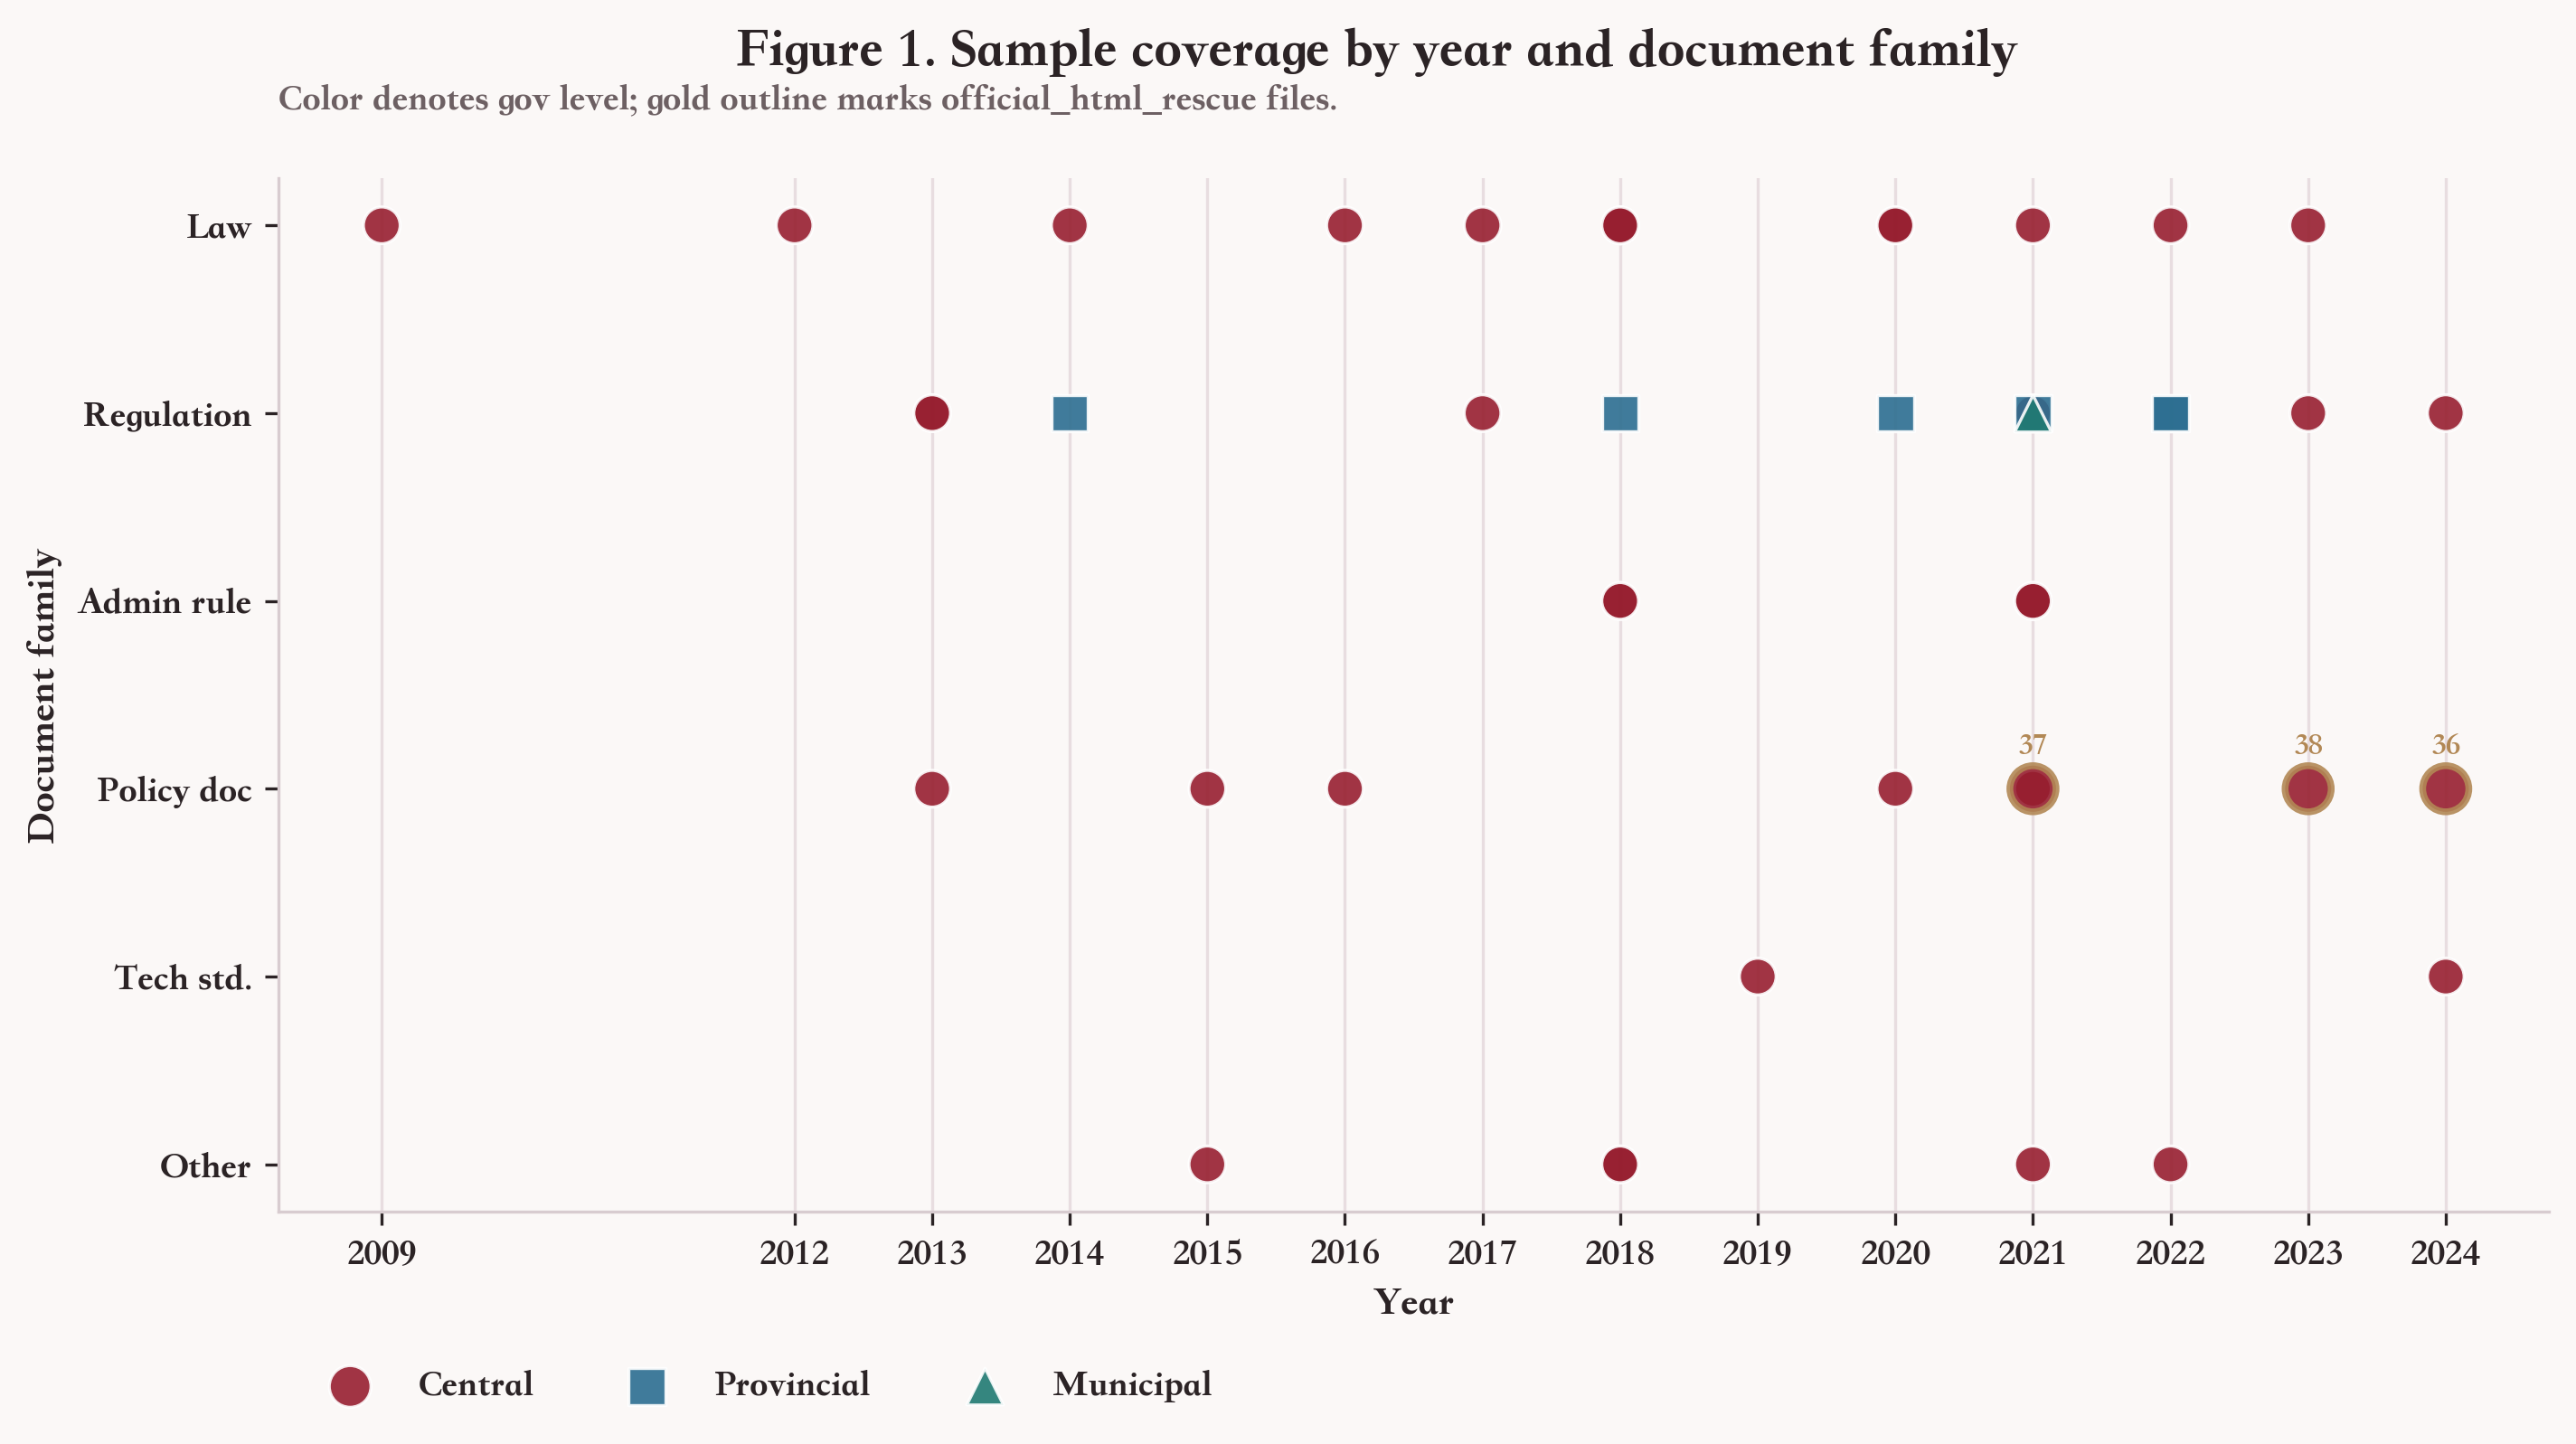
\includegraphics[width=0.98\textwidth]{../output/figures/prestudy_report/fig1_sample_timeline.png}
\caption{预调研样本的年份—文件类型分布}
\label{fig:sample_timeline}
\end{figure}

图 1 显示，2009---2024 年的样本覆盖围绕若干制度节点形成集聚：2013
年前后是大气治理行动计划与法律修订的重要阶段，2021---2024
年则更多出现双碳、绿色转型与地方生态环境条例的密集出台。样本中，法律与法规占据较高比重，规范性文件则集中承载行动计划、指导意见和综合部署类文本。

进一步看政策工具组合，当前样本呈现出十分清晰的``强管制骨架 +
多元工具嵌入''结构。

\begin{figure}[H]
\centering
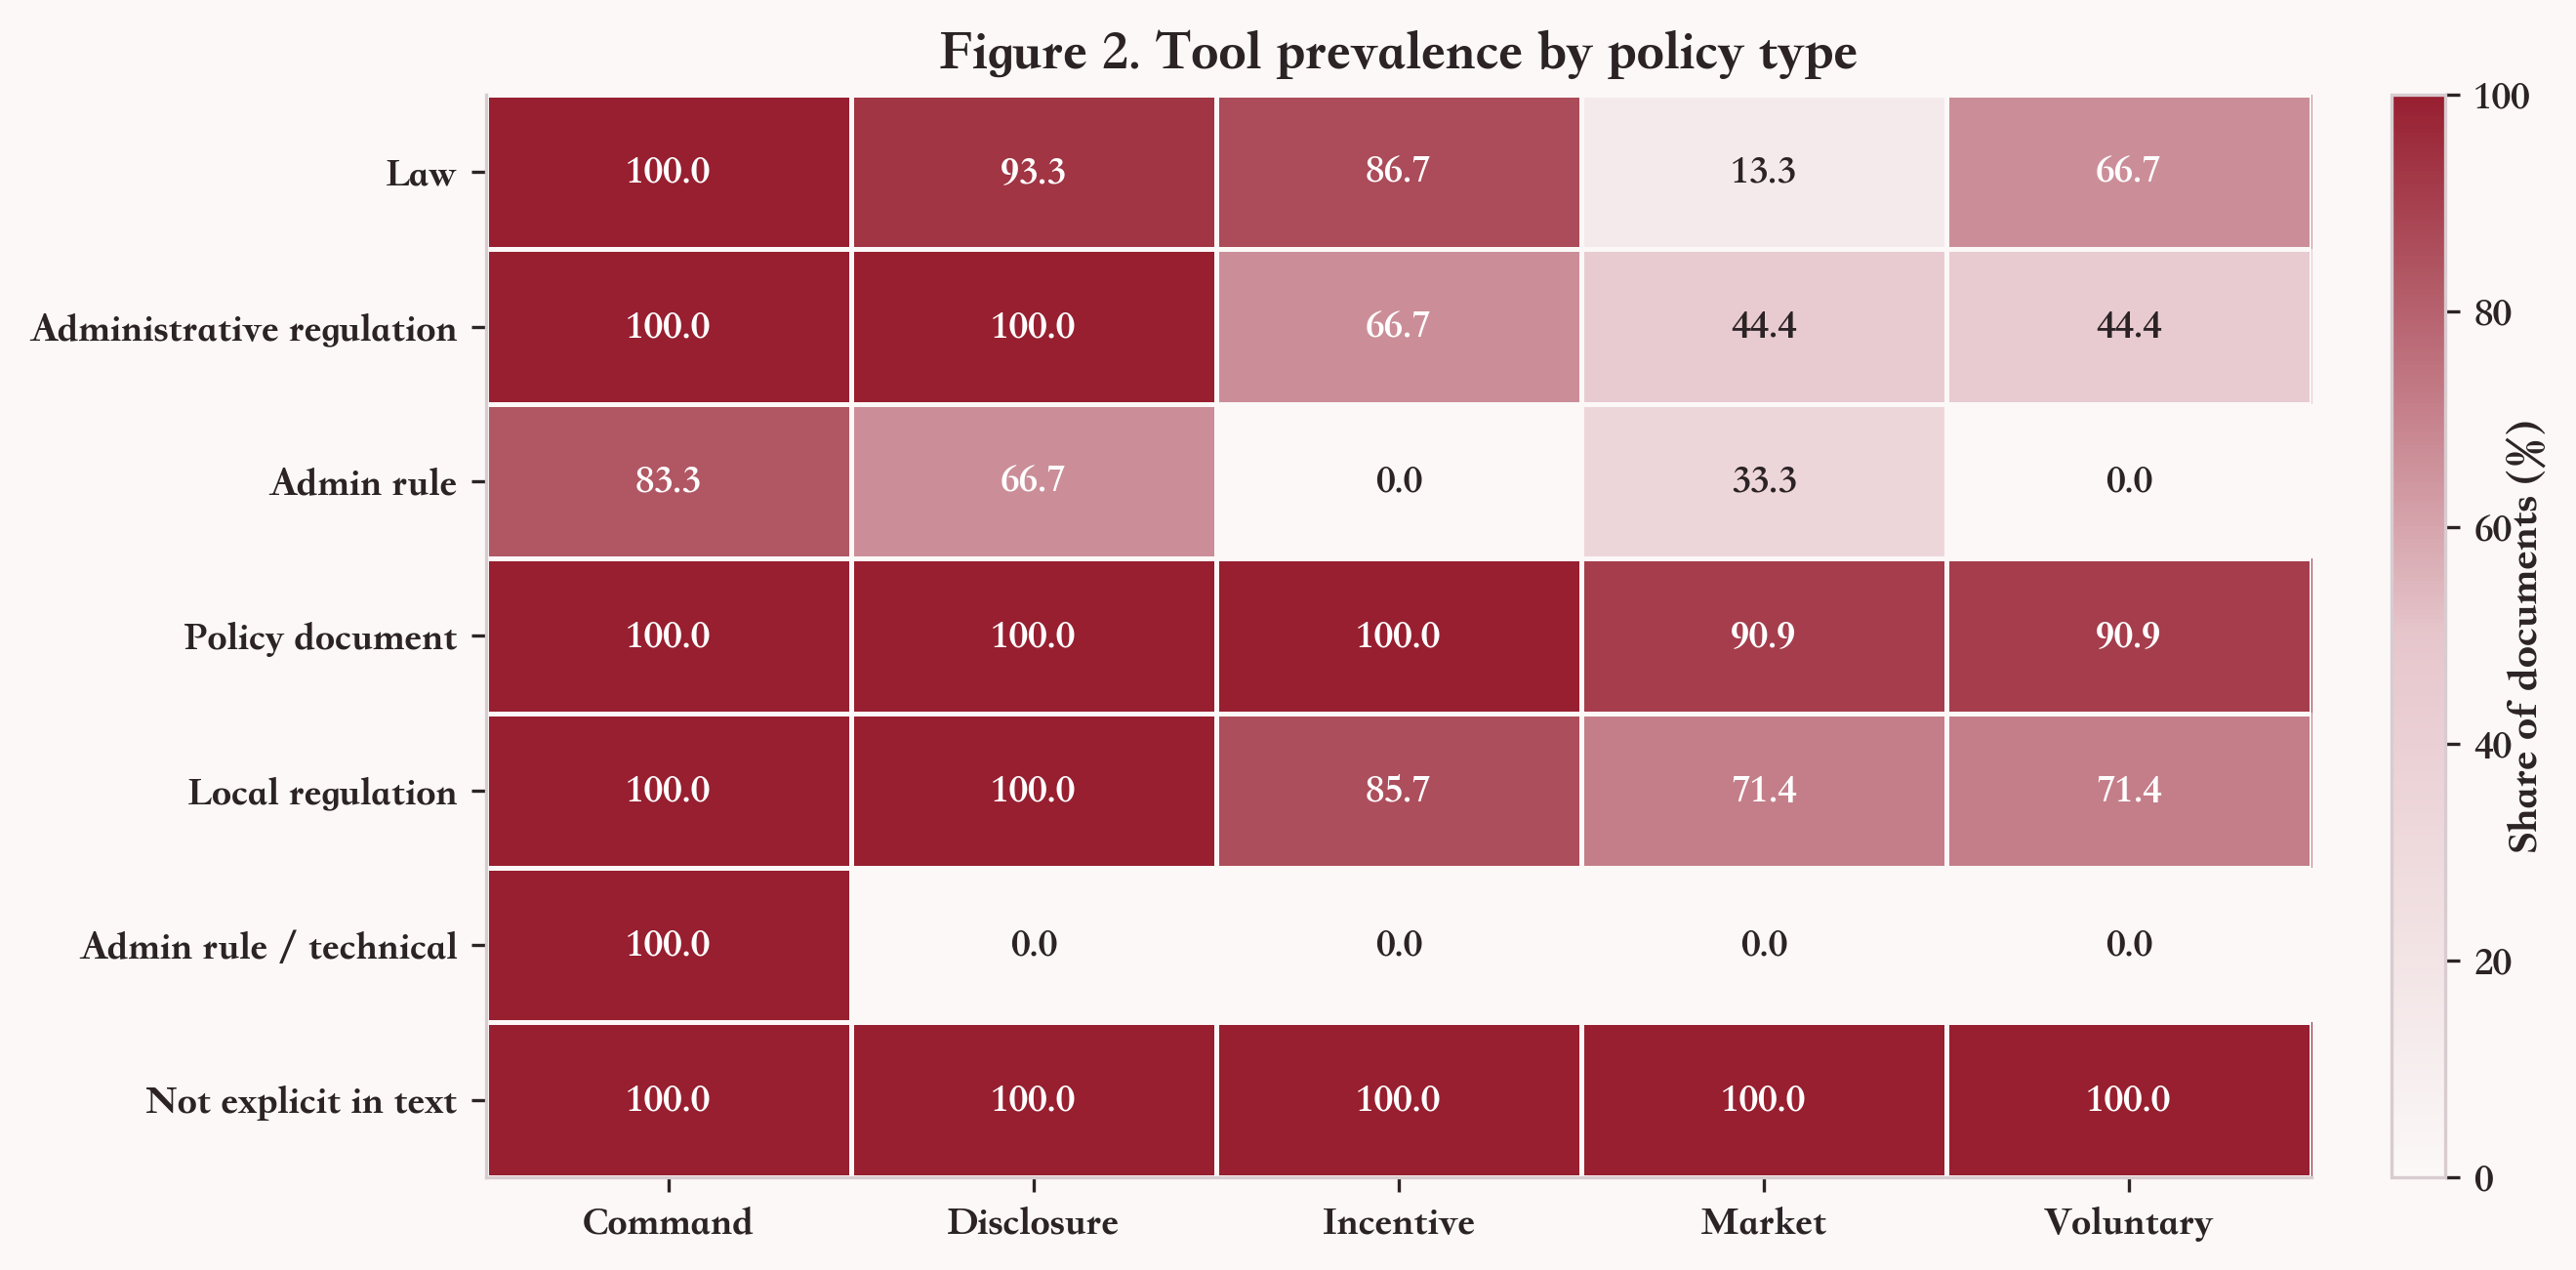
\includegraphics[width=0.96\textwidth]{../output/figures/prestudy_report/fig2_tool_heatmap.png}
\caption{不同政策类型中的政策工具覆盖率}
\label{fig:tool_heatmap}
\end{figure}

在全样本中，命令控制型工具覆盖率达 98\%，信息公开型工具达
92\%，经济激励型工具达 74\%，自愿型工具达 60\%，市场机制型工具为
48\%。这意味着，中国环境政策文本以强约束框架为骨架，并持续吸纳激励、市场与协同治理元素。其中，规范性文件和地方性法规往往呈现更完整的工具组合，说明综合性政策与地方立法更倾向于把多种治理手段并置于同一文本之中。

如果把视角从``工具类型''进一步推进到``政策任务结构''，样本差异会更加鲜明。

\begin{figure}[H]
\centering
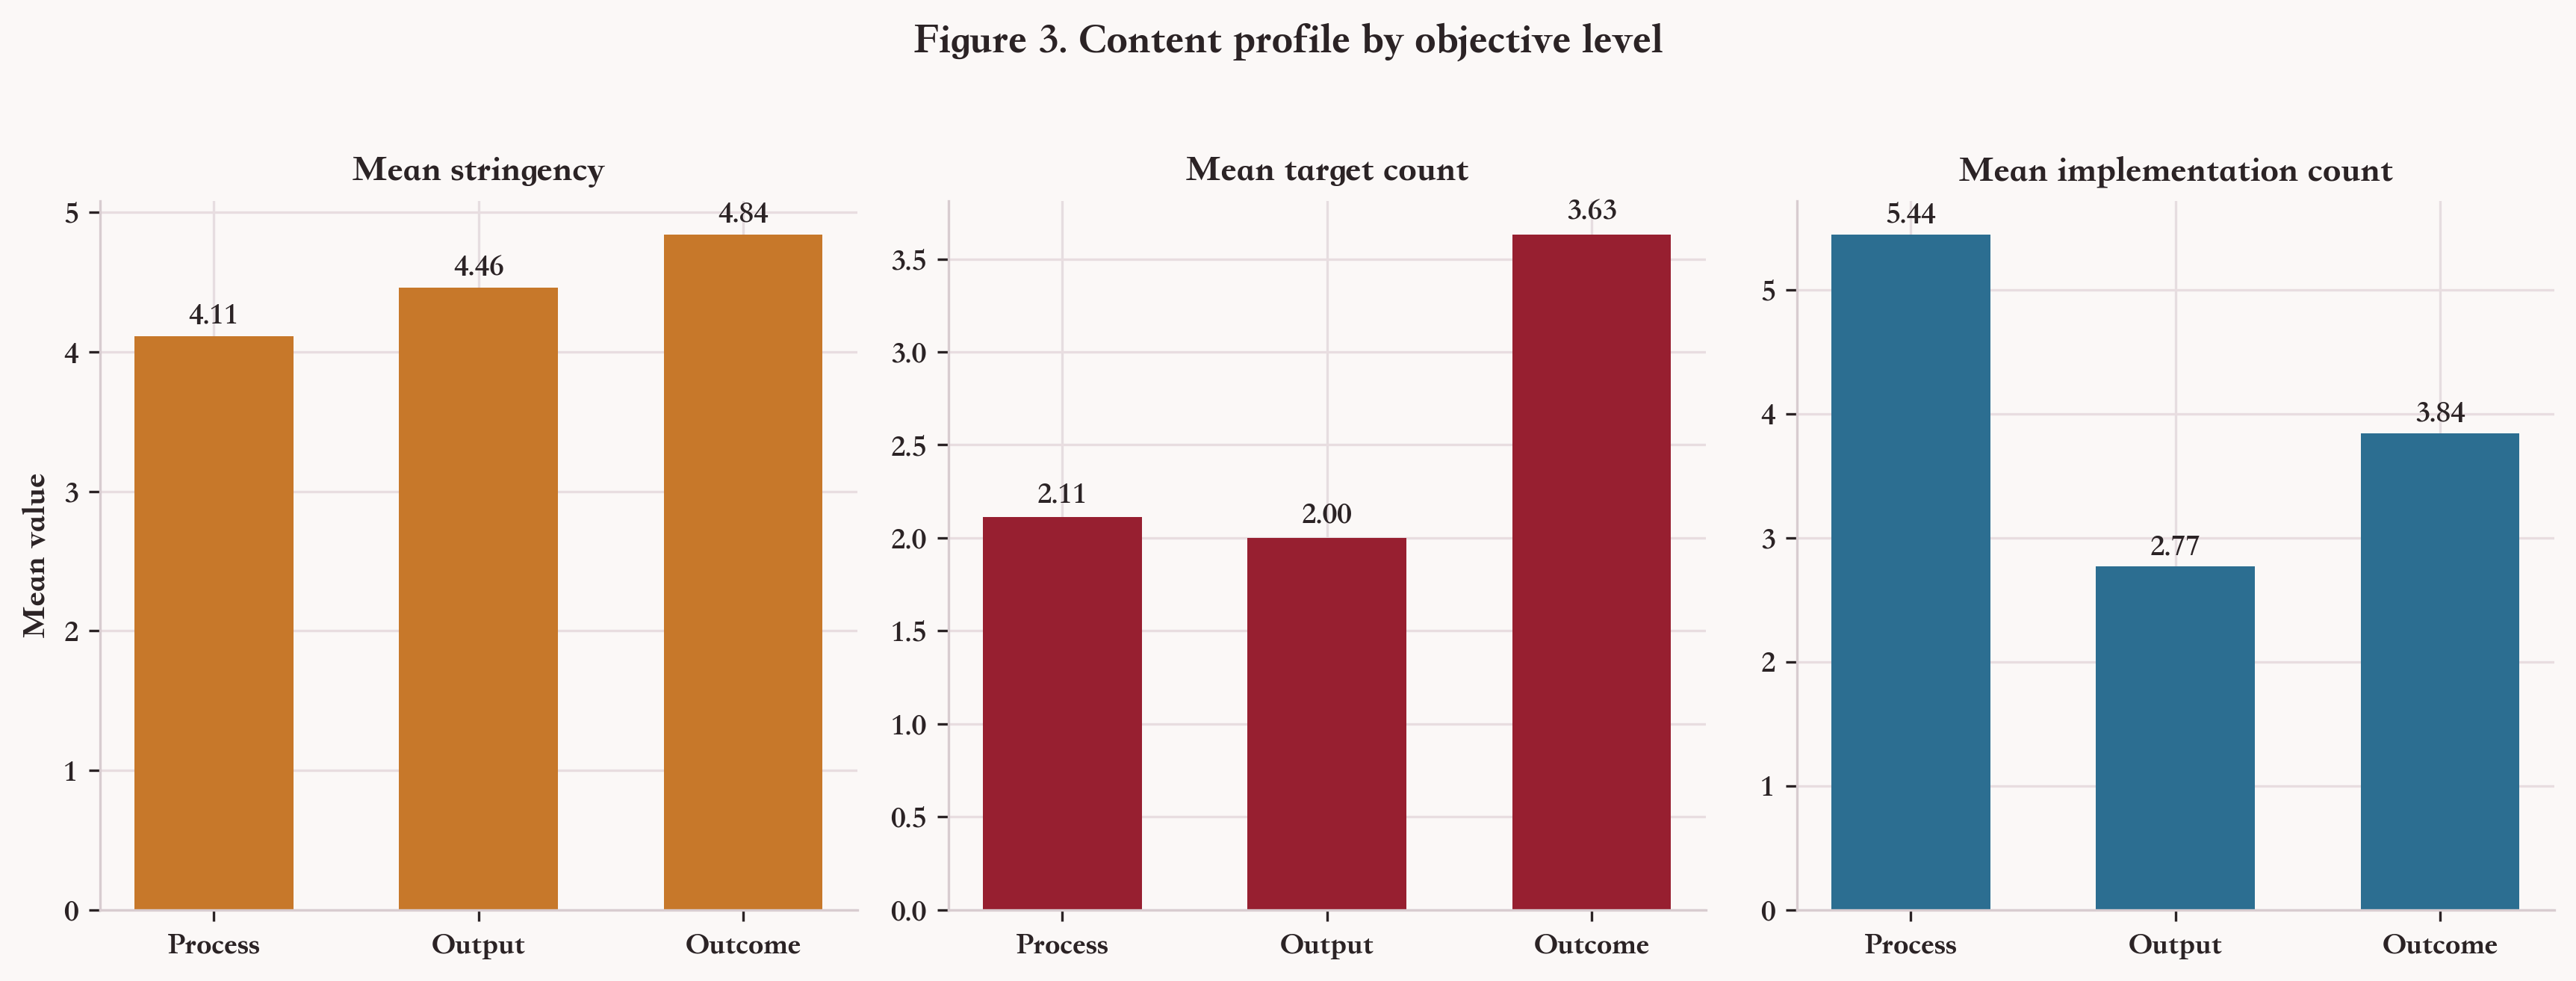
\includegraphics[width=0.98\textwidth]{../output/figures/prestudy_report/fig3_objective_profile.png}
\caption{不同目标层次文件的内容画像}
\label{fig:objective_profile}
\end{figure}

预调研样本中，结果型文件 19 份，过程型文件 18 份，产出型文件 13
份。结果型文件的平均规制严格度达到 4.84，平均量化目标数为
3.63，明显高于其他两类文件；过程型文件的平均执行机制数达到
5.44，为三类中最高；产出型文件则相对居中。这个分布很重要，因为它提示正式研究不宜只看``强弱''或``松严''，还应同时区分政策文本是在设定约束性结果目标，还是在搭建执行程序与组织安排。

按政府层级进一步比较，省级文件的平均执行机制数达到 6.83，中央文件为
3.84。地方文本通常比中央更``细''，这类差异正是后续识别中央---地方传导模式时最值得保留的文本信息。

\section{四、多模型抽取质量评估}

本轮预调研最核心的质量结论，是不同字段之间存在非常清晰的稳定性梯度。

\begin{figure}[H]
\centering
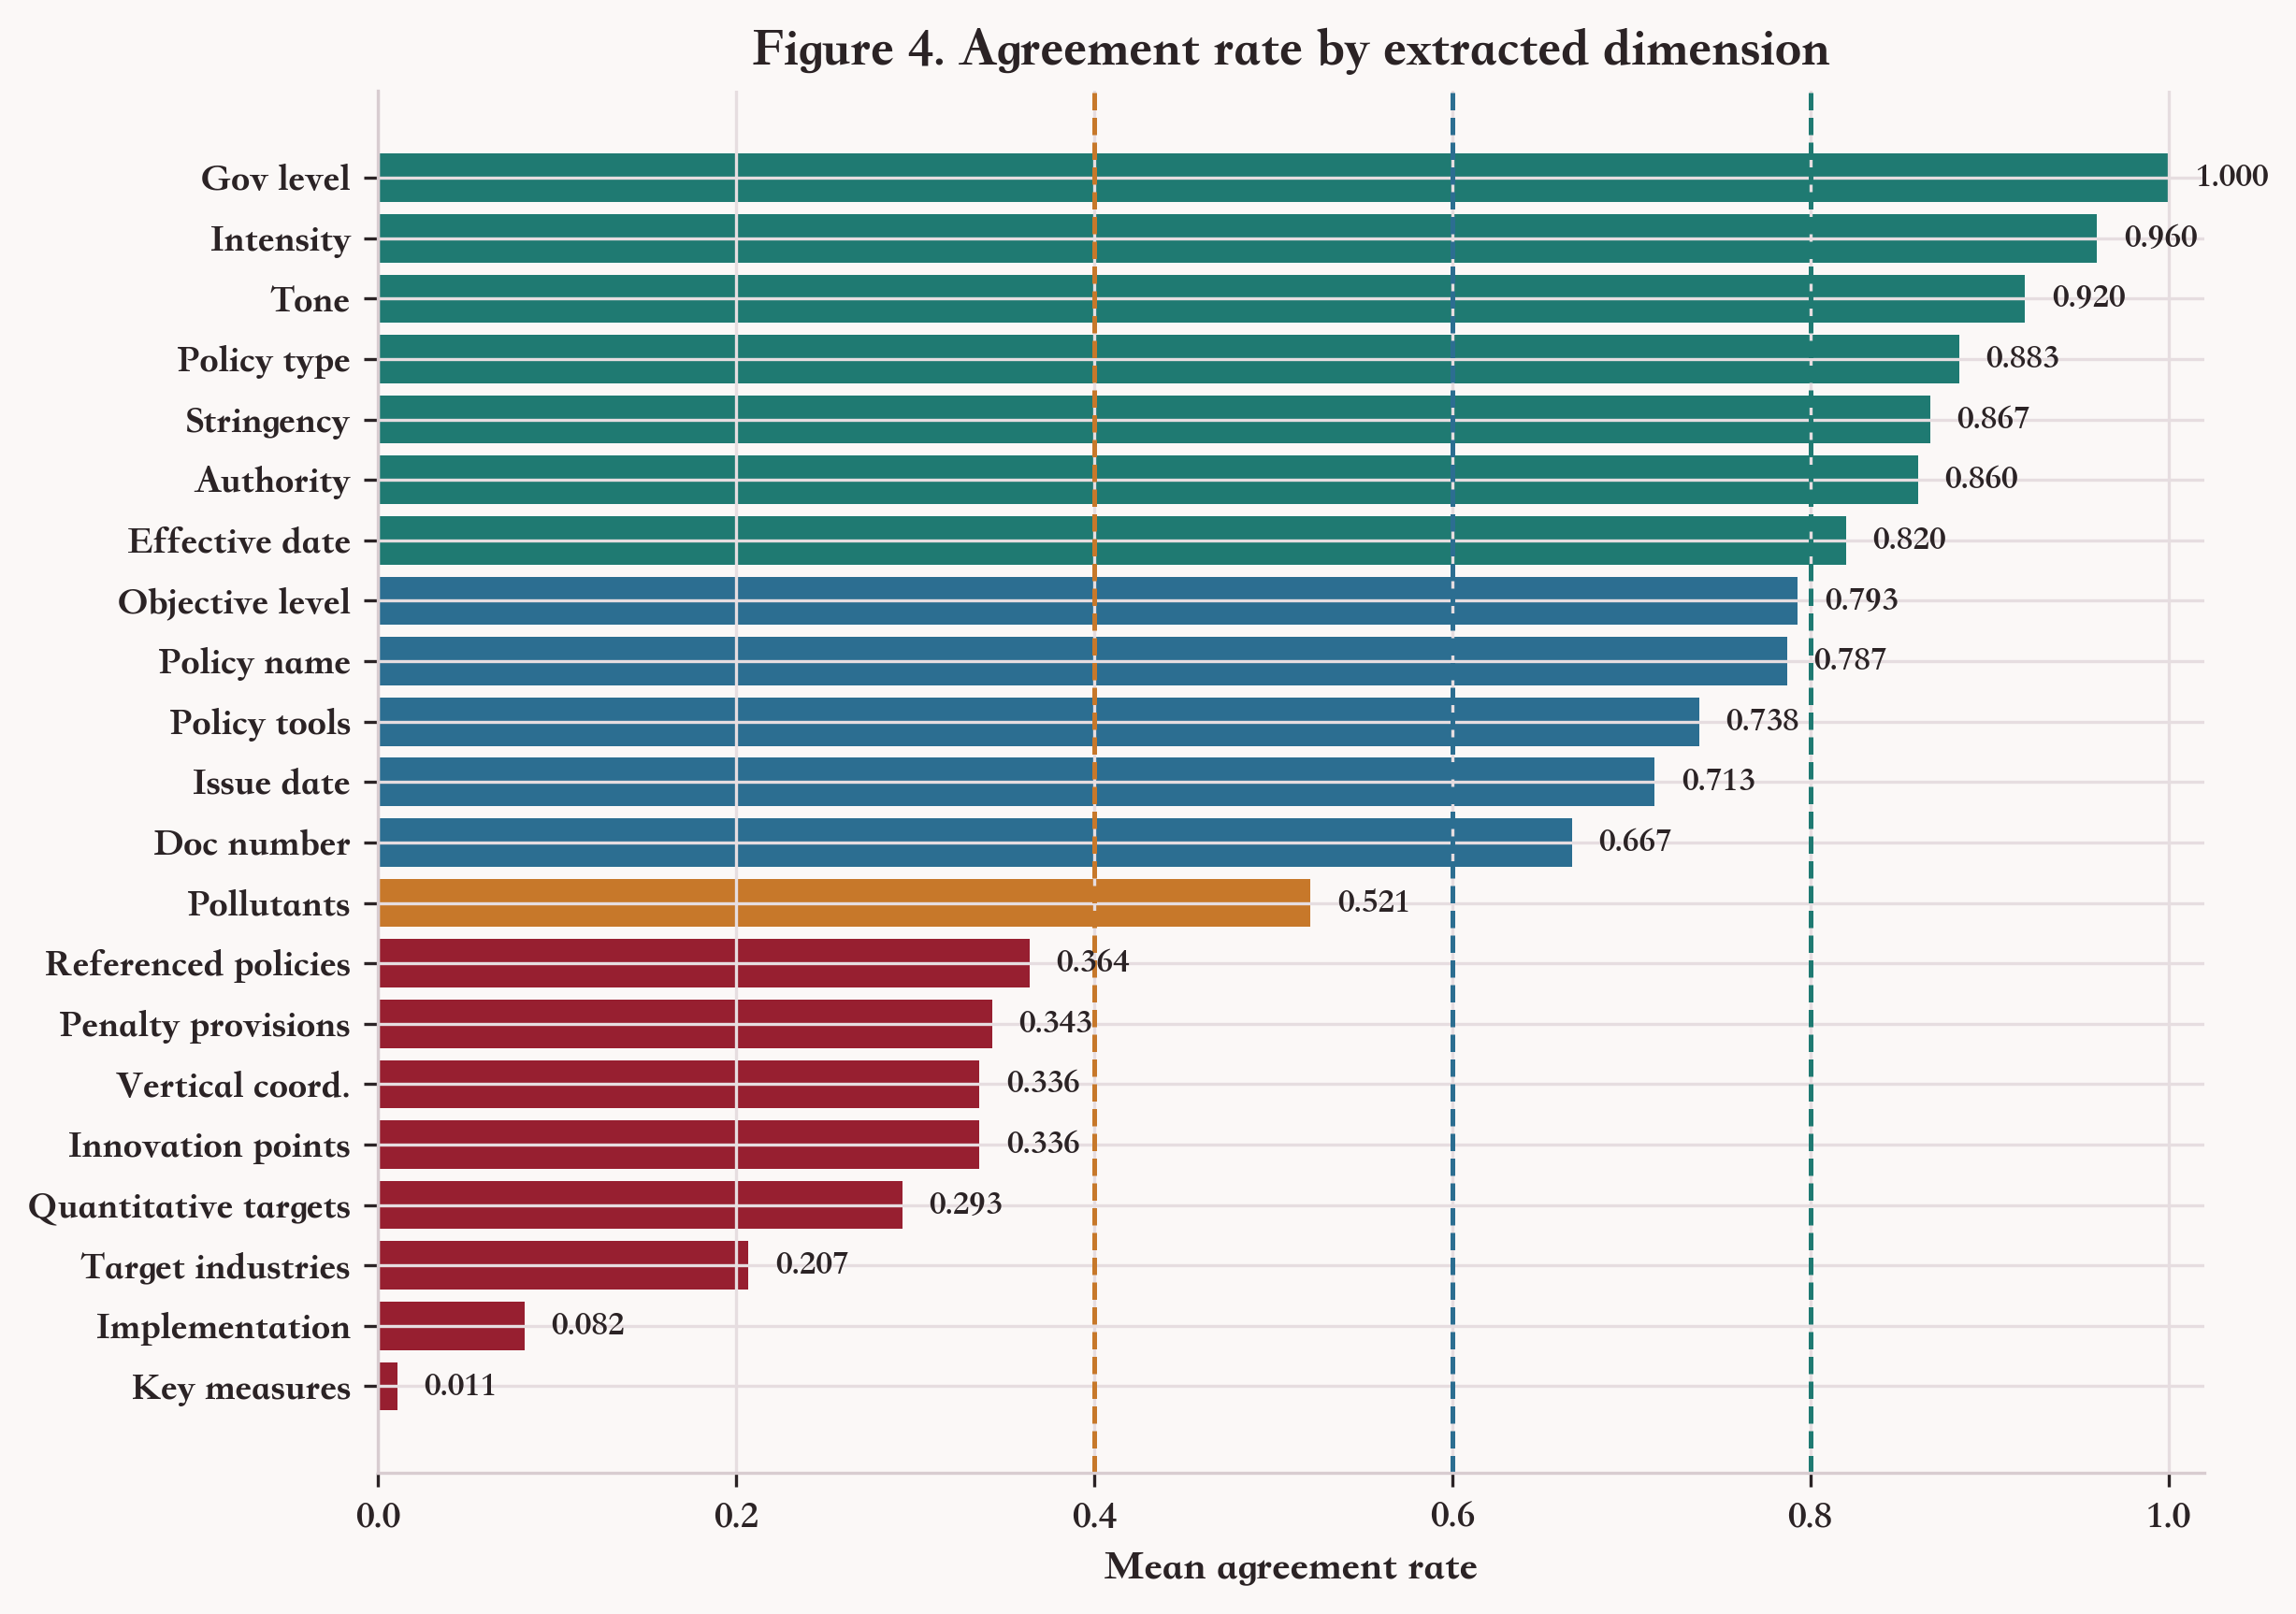
\includegraphics[width=0.98\textwidth]{../output/figures/prestudy_report/fig4_dimension_agreement.png}
\caption{各抽取维度的平均一致率}
\label{fig:dimension_agreement}
\end{figure}

从图 4
可以看到，政府层级、政策力度、政策语气、政策类型、规制严格度、发文机关、施行日期等制度属性的一致率已达到较高水平，其中政府层级为
1.000，政策力度为 0.960，政策语气为 0.920，政策类型为
0.883，规制严格度为
0.867。目标层次、政策名称、政策工具、发布日期与文号处于中等一致区间，也具备进一步规则化和扩样的基础。

真正的分水岭出现在开放式字段。关键措施的一致率仅为 0.011，执行机制为
0.082，目标行业为 0.207，量化目标为 0.293，创新点与纵向协调均为
0.336，引用政策为
0.364。分歧主要来自摘要、归纳、命名标准与边界划分上的差异，模型之间更容易在粒度和表达方式上出现偏离。因此，正式研究应把它们改造为规则化派生变量，例如执行机制密度、引用上位法数量、是否存在明确问责条款、是否存在区域联防联控安排等，而不宜直接把开放文本原值入模。

从文件层级看，当前结果也呈现出可解释的分布。

\begin{figure}[H]
\centering
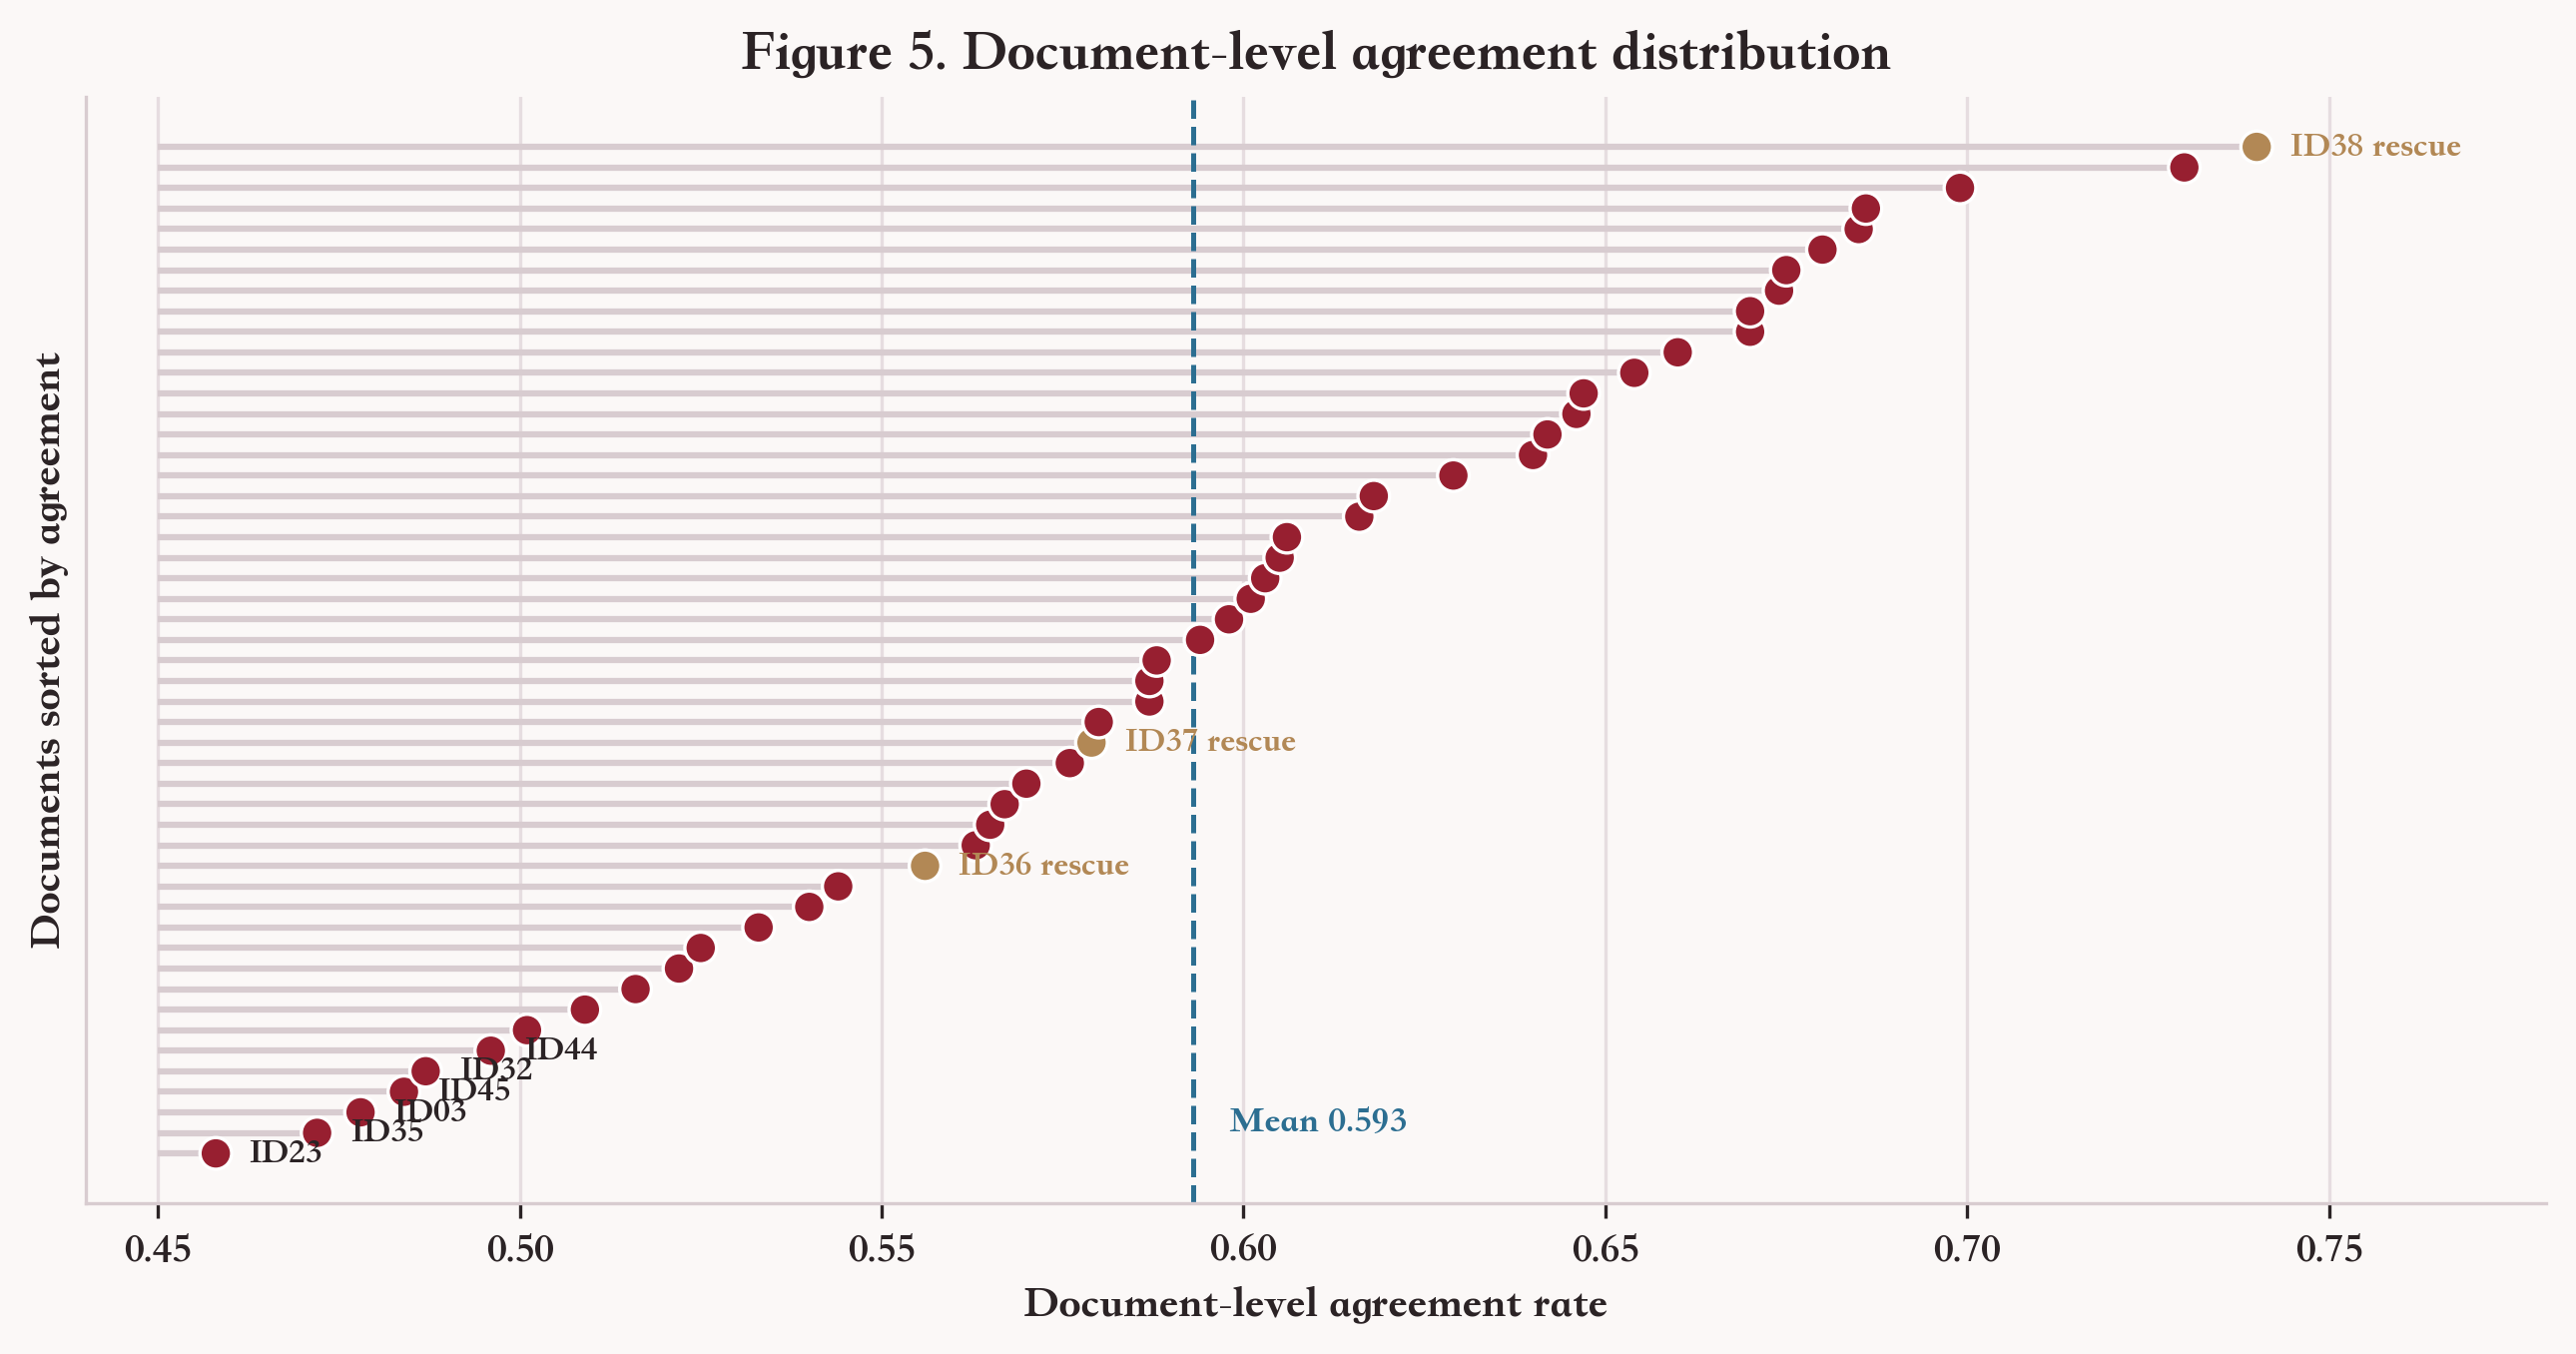
\includegraphics[width=0.98\textwidth]{../output/figures/prestudy_report/fig5_document_agreement.png}
\caption{文件层级总体一致率分布}
\label{fig:document_agreement}
\end{figure}

最低一致率文件包括《可再生能源法（2009
修正）》《关于构建现代环境治理体系的指导意见》《土壤污染防治行动计划》《上海市环境保护条例》《2030年前碳达峰行动方案》等。它们有一个共同特点：要么是综合性框架文本，要么是技术标准密集文本，要么是地方综合条例，因而在执行机制、创新点、目标行业与引用政策等开放字段上更容易拉开模型判断。相反，\path{official\_html\_rescue}
并未系统性拖累结果质量，三份补源文件中，《空气质量持续改善行动计划（2023）》的一致率反而达到
0.740，为全样本最高值。这说明，官方正文补源是一条可以继续使用的稳健路径。

据此，当前变量可以分为两类。第一类是已经可用于正式扩样与统计描述的稳定字段：\path{gov\_level}、\path{policy\_type}、\path{policy\_intensity}、\path{policy\_tone}、\path{regulatory\_stringency}、\path{policy\_objective\_level}、\path{policy\_tools}、\path{issue\_date}、\path{effective\_date}、\path{doc\_number}。第二类是应先进入规则化构造与人工核验的字段：\path{implementation\_mechanism}、\path{key\_measures}、\path{quantitative\_targets}、\path{innovation\_points}、\path{vertical\_coordination}、\path{referenced\_policies}、\path{penalty\_provisions}、\path{target\_industries}、\path{pollutant\_types}。

\section{五、政策内容的初步经验结构}

预调研的意义不只在于质量控制，也在于它已经显露出后续正式研究最值得追踪的几个经验维度。

\subsection{（一）强制性与严厉型文本占据主导}

50 份文件中，强制性文本 48 份，引导性文本仅 2 份；严厉型语气文件 39
份，中性语气文件 11 份；全样本平均规制严格度为
4.48。这说明环境政策文本以明确约束、责任传导与执行压力并存的制度风格为主。

\subsection{（二）结果型文件更强调``目标约束''，过程型文件更强调``执行布置''}

结果型文件的平均量化目标数为 3.63，平均规制严格度为
4.84；过程型文件的平均执行机制数为
5.44；产出型文件则处于两者之间。对正式研究而言，这意味着文本传导不能只理解为相似度问题，更应理解为``中央要求被地方翻译成什么样的任务结构''。

\subsection{（三）地方立法的工具箱更完整、执行机制更密集}

省级文件平均包含 4.17 类政策工具，高于中央文件的 3.65；平均执行机制数为
6.83，也显著高于中央文件的
3.84。地方文本更像是把上位制度要求嵌入地方治理程序，而不仅仅是复述中央口号。因此，后续正式研究完全可以围绕``地方是在做细化适配，还是在做形式复制''这一判断展开。

\subsection{（四）上位法引用网络已经形成清晰中心}

\begin{figure}[H]
\centering
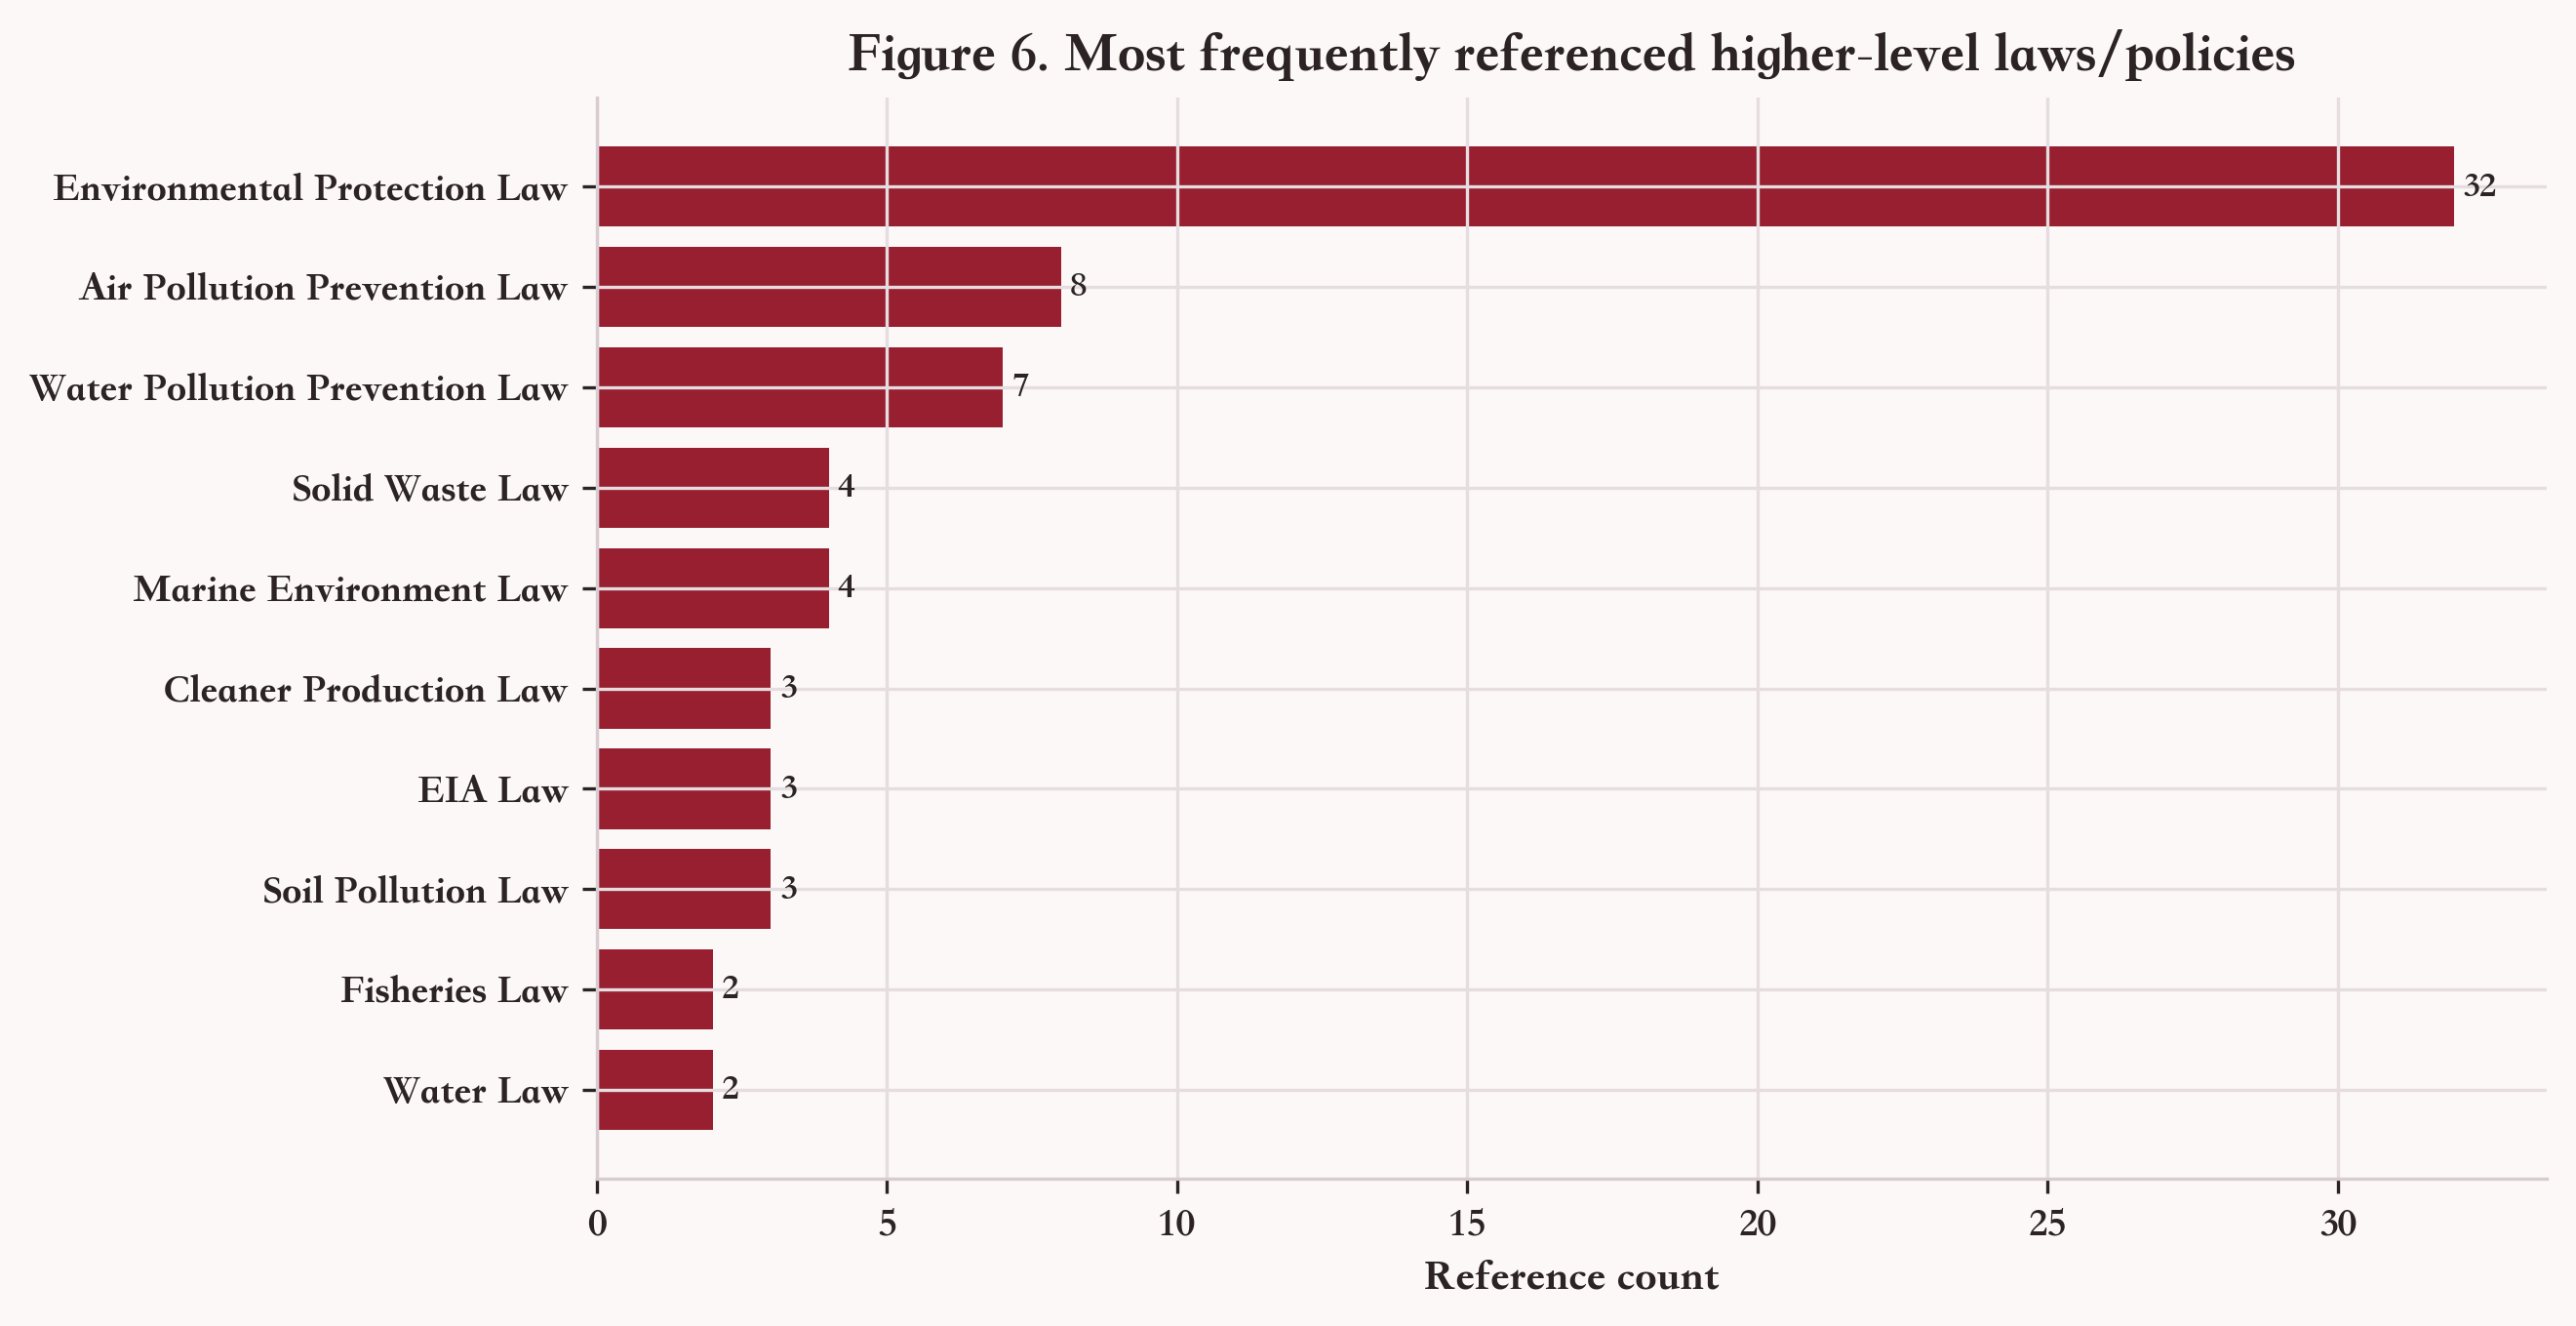
\includegraphics[width=0.96\textwidth]{../output/figures/prestudy_report/fig6_top_references.png}
\caption{样本中最常被引用的上位法/政策}
\label{fig:top_references}
\end{figure}

《中华人民共和国环境保护法》在 50 份样本中被引用 32
次，显著高于其他上位法，构成当前样本最强的制度锚点；《大气污染防治法》《水污染防治法》分别被引用
8 次和 7
次，构成污染治理领域最重要的专项法律支撑。这个结果意味着，后续完全可以把``上位法引用密度''\,``引用网络结构''作为正式研究中的关键文本指标。

\subsection{（五）执行机制有高度集中的制度语汇}

当前样本中出现频率最高的执行机制依次为排污许可制度（23
次）、目标责任考核（19 次）、环评审批（14 次）和总量控制（12
次）。这些高频机制已经可以进一步转化为问责、准入、配额、协同四类治理机制的基础语汇。正式研究中的机制维度无需从头发明，预调研样本已经给出了足够清晰的制度词汇表。

\section{六、典型个案剖析}

为了判断当前变量是否具有研究解释力，仅看全样本均值还不够，还需要回到具体文本观察其结构差异。

\textbf{1.《大气污染防治行动计划》（2013）}\\
该文件同时覆盖命令控制、经济激励、市场机制、信息公开与自愿型五类工具，规制严格度为
5，量化目标直接指向北京 PM2.5
水平，并同时嵌入环评审批、总量控制、目标责任考核、区域联防联控与排污许可等多种执行安排。它代表的是一种典型的``综合治理
+ 强目标约束''文本结构。

\textbf{2.《空气质量持续改善行动计划》（2023）}\\
这是三份补源文件中抽取质量最高的一份，一致率达到
0.740。其文本同时包含全国与重点区域目标，既有污染物减排指标，也有运输结构与能源结构调整目标，执行机制上继续保留总量控制、排污许可、环评审批、区域联防联控和责任考核。这个案例说明，官方网页补源完全可以服务于正式研究，不必把图像型
PDF 视为天然不可用样本。

\textbf{3.《关于推进污水资源化利用的指导意见》（2021）}\\
该文件同样采用五类工具并举的结构，但规制强度为
3，目标层次为产出型，执行机制明显少于大气治理类行动计划。这表明，在资源化利用与绿色转型类政策中，政策文本更强调设施建设、资源配置与市场化调节，而非单纯的高压问责。

\textbf{4.《上海市环境保护条例》（2022）}\\
该文件工具组合完整，执行机制多达 7
项，并出现按日连续处罚、区域协同保护、碳达峰碳中和纳入地方条例等内容，但总体一致率仅为
0.484。其低一致并不意味着文本质量低，而是说明地方综合条例常常把执行机制、创新点和地方裁量嵌入更复杂的制度表述之中，恰好是后续人工核验和规则化构造最值得优先处理的对象。

\section{七、阶段性判断与正式研究推进建议}

本轮预调研的结论可以压缩为三句话。

第一，\textbf{文本结构化主线已经跑通}。以政策层级、力度、语气、类型、规制强度、目标层次与工具组合为核心的制度属性，已经能够在多模型交叉抽取下形成稳定结果，完全可以进入正式样本扩展。

第二，\textbf{开放式字段不宜直接入模，但已经足以支撑规则化派生变量设计}。执行机制、关键措施、创新点、量化目标与纵向协调信息仍然很有价值，只是应先经过命名标准化、规则归并与人工核验，再转化为更适合统计分析的结构化指标。

第三，\textbf{正式研究的切入点已经相当清楚}。预调研最有解释力的方向，是考察中央治理信号进入地方文本后，究竟形成了怎样的工具组合、目标结构、问责安排与上位法引用网络；地方究竟是在做细化适配，还是在做形式复制。这一判断既来自理论问题，也已经得到预调研样本的经验支持。

基于上述结论，下一步工作建议按以下顺序推进：

\begin{enumerate}
\def\labelenumi{\arabic{enumi}.}
\tightlist
\item
  以当前稳定字段为基础扩展正式样本，优先保证时间、层级和政策类型覆盖。
\item
  以 \path{pilot\_validation\_sheet.csv}
  为入口，对低一致率文件和低一致率字段开展人工核验。
\item
  针对执行机制、引用政策、问责条款、量化目标等开放字段，建立规则化派生变量脚本。
\item
  在文本测量稳定后，再进入中央---地方相似度、政策扩散与后续外部结果匹配环节。
\end{enumerate}

\clearpage
\appendix
\section{复现入口与核心输出}

\subsection{1. 关键脚本}

\begin{itemize}
\tightlist
\item
  \path{scripts/analysis/02\_build\_prestudy\_validation\_sheet.py}
\item
  \path{scripts/analysis/04\_build\_prestudy\_report\_assets.py}
\end{itemize}

\subsection{2.
本轮核心输出}

\begin{itemize}
\tightlist
\item
  \path{output/tables/prestudy\_report/prestudy\_doc\_summary.csv}
\item
  \path{output/tables/prestudy\_report/prestudy\_dimension\_agreement.csv}
\item
  \path{output/tables/prestudy\_report/prestudy\_model\_quality.csv}
\item
  \path{output/tables/prestudy\_report/prestudy\_tool\_prevalence.csv}
\item
  \path{output/tables/prestudy\_report/prestudy\_top\_referenced\_policies.csv}
\item
  \path{output/tables/prestudy\_report/prestudy\_top\_implementation\_mechanisms.csv}
\item
  \path{output/figures/prestudy\_report/fig1\_sample\_timeline.png}
\item
  \path{output/figures/prestudy\_report/fig2\_tool\_heatmap.png}
\item
  \path{output/figures/prestudy\_report/fig3\_objective\_profile.png}
\item
  \path{output/figures/prestudy\_report/fig4\_dimension\_agreement.png}
\item
  \path{output/figures/prestudy\_report/fig5\_document\_agreement.png}
\item
  \path{output/figures/prestudy\_report/fig6\_top\_references.png}
\end{itemize}

\subsection{3. 复现命令}

\begin{CodeBlock}
python3 scripts/analysis/02_build_prestudy_validation_sheet.py
MPLCONFIGDIR=.mplconfig python3 scripts/analysis/04_build_prestudy_report_assets.py
\end{CodeBlock}

\subsection{4. AI 使用说明}

本报告的数据整理、图表生成在研究者监督下借助 AI
完成；所有统计判断均直接对应于本仓库保存的结构化结果、图表脚本与原始抽取输出，未新增任何未运行、未落盘或不可回溯的结论。


\end{document}
